%-%-%-%-%-%-%-%-%-%-%-%-%-%-%-%-%-%-%-%-%-%-%-%-%-%-%-%-%-%-%-%-%-%-%-%-%-%-%
%%% MAIN DOCUMENT %%%

%-%-%-%-%-%-%-%-%-%-%-%-%-%-%-%-%-%-%-%-%-%-%-%-%-%-%-%-%-%-%-%-%-%-%-%-%-%-%

\documentclass[12pt, oneside]{book}
\usepackage{xcolor}
\usepackage{minted}

% \usepackage[T1]{fontenc}

\usepackage{draculatheme}
\newcommand{\documentTheme}{draculafg}
\newcommand{\documentLogo}{../../images/small logo_white.png}
\newcommand{\documentBigLogo}{../../images/logo_white_text.png}
\usemintedstyle{dracula}

\usemintedstyle{dracula}

\setminted{
    linenos=true,
    numbersep=5pt,
    frame=lines,
    framesep=2mm,
    breaklines=true
}

% \newcommand{\documentBigLogo}{../../images/Hendrix Logo.png}
% \newcommand{\documentLogo}{../../images/small logo.png}
% \newcommand{\documentTheme}{black}

%%% AESTHETICS %%%
%-%-%-%-%-%-%-%-%-%-%-%-%-%-%-%-%-%-%-%-%-%-%-%-%-%-%-%-%-%-%-%-%-%-%-%-%-%-%


%%% Dimensions and Spacing %%%
\usepackage[margin=1in]{geometry}
\setlength{\parindent}{0pt}
\usepackage{setspace}
\usepackage{mathtools}
\usepackage{esint}
\usepackage{adjustbox}
\linespread{1}
\usepackage{listings}
\usepackage{tikz}
\usetikzlibrary{shapes,backgrounds,calc,patterns,positioning}
\usepgflibrary{shadings}
\usepackage{pgfkeys}
\usepackage{pdftexcmds}
\usepackage{shellesc}
\usepackage{algorithm, algorithmic, xspace}
%%% Define new colors %%%
\definecolor{orangehdx}{rgb}{0.96, 0.51, 0.16}

% Normal colors
\definecolor{xred}{HTML}{BD4242}
\definecolor{xblue}{HTML}{4268BD}
\definecolor{xgreen}{HTML}{52B256}
\definecolor{xpurple}{HTML}{7F52B2}
\definecolor{xorange}{HTML}{FD9337}
\definecolor{xdotted}{HTML}{999999}
\definecolor{xgray}{HTML}{777777}
\definecolor{xcyan}{HTML}{80F5DC}
\definecolor{xpink}{HTML}{F690EA}
\definecolor{xgrayblue}{HTML}{49B095}
\definecolor{xgraycyan}{HTML}{5AA1B9}

% Dark colors
\colorlet{xdarkred}{red!85!black}
\colorlet{xdarkblue}{xblue!85!black}
\colorlet{xdarkgreen}{xgreen!85!black}
\colorlet{xdarkpurple}{xpurple!85!black}
\colorlet{xdarkorange}{xorange!85!black}
\definecolor{xdarkcyan}{HTML}{008B8B}
\colorlet{xdarkgray}{xgray!85!black}

% Very dark colors
\colorlet{xverydarkblue}{xblue!50!black}

% Document-specific colors
\colorlet{normaltextcolor}{black}
\colorlet{figtextcolor}{xblue}

% Enumerated colors
\colorlet{xcol0}{black}
\colorlet{xcol1}{xred}
\colorlet{xcol2}{xblue}
\colorlet{xcol3}{xgreen}
\colorlet{xcol4}{xpurple}
\colorlet{xcol5}{xorange}
\colorlet{xcol6}{xcyan}
\colorlet{xcol7}{xpink!75!black}

% Blue-Purple (should just used colorbrewer...)
\definecolor{xrainbow0}{HTML}{e41a1c}
\definecolor{xrainbow1}{HTML}{a24057}
\definecolor{xrainbow2}{HTML}{606692}
\definecolor{xrainbow3}{HTML}{3a85a8}
\definecolor{xrainbow4}{HTML}{42977e}
\definecolor{xrainbow5}{HTML}{4aaa54}
\definecolor{xrainbow6}{HTML}{629363}
\definecolor{xrainbow7}{HTML}{7e6e85}
\definecolor{xrainbow8}{HTML}{9c509b}
\definecolor{xrainbow9}{HTML}{c4625d}
\definecolor{xrainbow10}{HTML}{eb751f}
\definecolor{xrainbow11}{HTML}{ff9709}

%------- %
% XHFILL %
%------- %



%%% Chapter Headings %%%

\newcommand{\gradientrule}{
    \begin{tikzpicture}
        \shade[left color=orangehdx, right color=black, middle color=gray] (0,0) rectangle (\linewidth,0.4pt);
    \end{tikzpicture}
}

\usepackage[Glenn]{fncychap}
\ChTitleVar{\bfseries\scshape\color{\documentTheme}} % Needed for Dracula theme
\ChNumVar{\large\selectfont\color{\documentTheme}} % Needed for Dracula theme
\ChNameVar{\large\color{\documentTheme}} % Needed for Dracula theme
\usepackage{xpatch}


\xpatchcmd\DOCH
{\mghrulefill}{\color{orangehdx}\mghrulefill}
{}{\PatchFailed}
\xpatchcmd\DOTI
{\mghrulefill}{\color{orangehdx}\mghrulefill}
{}{\PatchFailed}
\xpatchcmd\DOTIS
{\mghrulefill}{\color{orangehdx}\mghrulefill}
{}{\PatchFailed}



%% Change Chapter Heading Placement %%
\usepackage{etoolbox}
\makeatletter
\patchcmd{\@makechapterhead}{\vspace*{50\p@}}{\vspace*{-20\p@}}{}{}
\patchcmd{\@makeschapterhead}{\vspace*{50\p@}}{\vspace*{-20\p@}}{}{}
\patchcmd{\DOTI}{\vskip 80\p@}{\vskip 40\p@}{}{}
\patchcmd{\DOTIS}{\vskip 40\p@}{\vskip 0\p@}{}{}
\makeatother



\renewcommand{\thesection}{\thechapter.\arabic{section}} %% Chapter.Section Numbering


%%% listingS %%%
\usepackage{graphicx}  
% \numberwithin{listing}{section}
\usepackage{float}
\usepackage{caption}

%%% Hyperlinks %%%
\usepackage{hyperref}
\definecolor{horange}{HTML}{f58026}
\hypersetup{
	colorlinks=true,
	linkcolor=horange,
	filecolor=horange,      
	urlcolor=horange,
}

\newcommand{\assignmentname}{Homework 3: Chapters 2 \& 3}

%% Headers and Footers %%
\usepackage{fancyhdr} % This should be set AFTER setting up the page geometry
\pagestyle{fancy} % options: empty , plain , fancy
\fancyhead[R]{\textcolor{draculafg}{\assignmentname}}
\fancyhead[L]{\textcolor{draculafg}{Hendrix College}}
\fancyhead[C]{\includegraphics[height=.50cm]{\documentLogo}} % Use for Dracula
\usepackage{xpatch}
\xpretocmd\headrule{\color{orangehdx}}{}{\PatchFailed}
\setlength{\footskip}{0.5in}
\setlength{\headheight}{18.5764pt}


%%%%% Colored Boxes %%%%%
\usepackage{tcolorbox}
\tcbuselibrary{skins}
\tcbuselibrary{theorems}
% \tcbuselibrary{minted}
\newcounter{BoxCounter}
\usepackage{dingbat}

%-%-%-%-%-%-%-%-%-%-%-%-%-%-%-%-%-%-%-%-%-%-%-%-%-%-%-%-%-%-%-%-%-%-%-%-%-%-%

%% MATH PACKAGES, ENVIRONMENTS, COMMANDS %%
%-%-%-%-%-%-%-%-%-%-%-%-%-%-%-%-%-%-%-%-%-%-%-%-%-%-%-%-%-%-%-%-%-%-%-%-%-%-%
%You'll need your own packages, theorem types, and commands.

\usepackage{fix-cm}
\usepackage{amsmath,amsthm} 
\usepackage{array, makecell}
\usepackage{colortbl}
\newcommand{\thickvrule}{\vrule width 1pt}

\newcommand{\thickhrule}{\Xhline{1pt}}

\usepackage{mathtools}
\usepackage{amssymb}
\usepackage[framemethod=tikz]{mdframed}
\usepackage{mathrsfs}
\usepackage{changepage}
\usepackage{multicol}
\usepackage{slashed}
\usepackage{enumerate}
\usepackage{braket}
\usepackage{booktabs}
\usepackage{enumitem}
\usepackage{kantlipsum}  %This package lets us generate random text for example purposes.
\usepackage{pgfplots}


%%% Custom Commands %%%
% Natural Numbers 
\newcommand{\N}{\mathbb{N}}

% Whole Numbers
\newcommand{\W}{\mathbb{W}}

% Integers
\newcommand{\Z}{\mathbb{Z}}

% Rational Numbers
\newcommand{\Q}{\mathbb{Q}}

% Real Numbers
\newcommand{\R}{\mathbb{R}}

% Complex Numbers
\newcommand{\C}{\mathbb{C}}

\newcommand{\I}{\mathbb{I}}

\newcommand{\pfs}{\noindent\makebox[\linewidth]{\rule{\textwidth}{0.4pt}}\vspace{0.5cm}}

\newcommand{\mysqrt}[1]{%
	\mathpalette\foo{#1}%
}
\newcommand{\dmysqrt}[1]{%
	\mathpalette\foodisplay{#1}%
}

% !TeX spellcheck = off
\newcommand{\foo}[2]{%
	% #1: math style, #2: content
	\sbox0{$#1\sqrt{#2}$}% Measure the size of the standard sqrt in the current style
	\begin{tikzpicture}[baseline=(sqrt.base)]
		\node[inner sep=0, outer sep=0] (sqrt) {$#1\sqrt{#2}$}; % Use the current math style
		\draw([yshift=-0.045em]sqrt.north east) -- ++(0,-0.5ex); % Draw the tick
	\end{tikzpicture}%
}
% !TeX spellcheck = off
\newcommand{\foodisplay}[2]{%
	% #1: math style, #2: content
	\sbox0{$#1\sqrt{#2}$}% Measure the size of the standard sqrt in the current style
	\begin{tikzpicture}[baseline=(sqrt.base)]
		\node[inner sep=0, outer sep=0] (sqrt) {$\displaystyle\sqrt{#2}$}; % Force displaystyle
		\draw[line width=0.4pt] ([yshift=-0.044em]sqrt.north east) -- ++(0,-0.5ex); % Draw the tick
	\end{tikzpicture}%
}

\renewcommand{\theenumi}{\arabic{enumi}}
\renewcommand{\labelenumi}{\textbf{\theenumi}.}

% \newcommand{}{\marginnote{
\includegraphics[width=2em]{caution.png}}}

\newmdenv[
	topline=false,
	bottomline=true,
	rightline=false,
	leftline=true,
	linewidth=1.5pt,
	linecolor=black, % default color, will be overridden in custom commands
	backgroundcolor=draculabg, % Needed for Dracula theme
	fontcolor=\documentTheme, % Needed for Dracula theme
	innertopmargin=0pt,
	innerbottommargin=5pt,
	innerrightmargin=10pt,
	innerleftmargin=10pt,
	leftmargin=0pt,
	rightmargin=0pt,
	skipabove=\topsep,
	skipbelow=\topsep,
]{customframedproof}

\newenvironment{proofpart}[2][black]{
    \begin{mdframed}[
        topline=false,
        bottomline=false,
        rightline=false,
        leftline=true,
        linewidth=1pt,
        linecolor=#1!40, % Custom color
        % innertopmargin=10pt,
        % innerbottommargin=10pt,
        innerleftmargin=10pt,
        innerrightmargin=10pt,
        leftmargin=0pt,
        rightmargin=0pt,
        % skipabove=\topsep,
        % skipbelow=\topsep%
    ]
    \noindent
    \begin{minipage}[t]{0.08\textwidth}%
        \textbf{#2}%
    \end{minipage}%
    \begin{minipage}[t]{0.90\textwidth}%
        \begin{adjustwidth}{0pt}{0pt}%
}{
    \end{adjustwidth}
    \end{minipage}
    \end{mdframed}
}

% Define a new environment 'proofscratch' for Proof and Scratch Paper
\newenvironment{proofscratch}[2]{%
    \begin{mdframed}[
        topline=false,
        bottomline=false,
        rightline=false,
        leftline=false,
        backgroundcolor=draculabg, % Background color for Dracula theme
        fontcolor=\documentTheme,       % Font color for Dracula theme
        innerleftmargin=-6pt,
        innertopmargin=0pt,
        leftmargin=0pt,
        rightmargin=0pt,
        skipabove=\topsep,
        skipbelow=\topsep,
    ]
    % % Begin TikZ picture for the vertical dotted line
    % \begin{tikzpicture}[overlay, remember picture]
    %     % Draw a vertical dotted line at approximately the center of the mdframed width
    %     \draw[dotted, thick] ([xshift=0.005\linewidth]current bounding box.north west) -- ([xshift=0.005\linewidth]current bounding box.south west);
    % \end{tikzpicture}%
    % % Create the left minipage for Proof
    \begin{minipage}[t]{0.47\textwidth}%
        \noindent\textit{Proof.} #1 \hfill \(\qed\)
    \end{minipage}%
    \hfill
    % Create the right minipage for Scratch Paper
    \begin{minipage}[t]{0.47\textwidth}%
        \textit{Scratch Paper.} #2
    \end{minipage}%
}{
    \end{mdframed}
}

\newenvironment{tipbox}
	{%
		\par\noindent%
		% Top dashed line (using \textwidth)
		\tikz[baseline]{\draw[dash pattern=on 3pt off 2pt, line width=0.5pt, color=draculapurple] (0,0) -- (\textwidth,0);}%
		\par\vspace{0.65em}%
		\noindent\textbf{\textcolor{draculapurple}{TIP:}}\quad%
	}
	{%
		\par%
		% Bottom dashed line
		\noindent%
		\tikz[baseline]{\draw[dash pattern=on 3pt off 2pt, line width=0.5pt, color=draculapurple] (0,0) -- (\textwidth,0);}%
		\par\vspace{0.35em}
	}

\newenvironment{notebox}
	{%
		\par\noindent%
		% Top dashed line (using \textwidth)
		\tikz[baseline]{\draw[dash pattern=on 3pt off 2pt, line width=0.5pt, color=draculagreen] (0,0) -- (\textwidth,0);}%
		\par\vspace{0.65em}%
		\noindent\textbf{\textcolor{draculagreen}{NOTE:}}\quad%
	}
	{%
		\par%
		% Bottom dashed line
		\noindent%
		\tikz[baseline]{\draw[dash pattern=on 3pt off 2pt, line width=0.5pt, color=draculagreen] (0,0) -- (\textwidth,0);}%
		\par\vspace{0.35em}
	}

\newenvironment{warningbox}
	{%
		\par\noindent%
		% Top dashed line (using \textwidth)
		\tikz[baseline]{\draw[dash pattern=on 3pt off 2pt, line width=0.5pt, color=draculared] (0,0) -- (\textwidth,0);}%
		\par\vspace{0.65em}%
		\noindent\textbf{\textcolor{draculared}{WARNING:}}\quad%
	}
	{%
		\par%
		% Bottom dashed line
		\noindent%
		\tikz[baseline]{\draw[dash pattern=on 3pt off 2pt, line width=0.5pt, color=draculared] (0,0) -- (\textwidth,0);}%
		\par\vspace{0.35em}
	}

\newenvironment{solution}{\textit{Solution.}}

\newcommand{\sol}[1]{
    \begin{customframedproof}[linecolor=orangehdx!75,]
        \begin{solution}
        #1
        \end{solution}
    \end{customframedproof}
}

\newcommand{\pf}[1]{
    \begin{customframedproof}[linecolor=orangehdx!75]
        \begin{proof}
        #1
        \end{proof}
    \end{customframedproof}
}

\def \proofDistance {10pt}

\newcommand{\disabs}[1]{\ensuremath{\left|#1\right|}}
\newcommand{\limn}{\lim_{n \rightarrow \infty}}
\newcommand{\limx}[2]{\lim_{x \rightarrow #1}#2}

\newcommand{\limc}[1]{\lim_{x \rightarrow c}#1}

\newcommand{\ninn}{n \in \N}

\newcommand{\mb}[1]{\mathbf{#1}}

\newcommand{\limsupn}[1]{\limsup_{n\rightarrow \infty}#1}
\newcommand{\liminfn}[1]{\liminf_{n\rightarrow \infty}#1}


\newcommand{\proj}{\text{proj}}

\newcommand{\p}{\partial}

\newcommand{\dydx}{\frac{dy}{dx}}
\newcommand{\dxdy}{\frac{dx}{dy}}
\newcommand{\dydt}{\frac{dy}{dt}}
\newcommand{\dxdt}{\frac{dx}{dt}}
\newcommand{\dzdt}{\frac{dz}{dt}}

\newcommand{\barNotationT}[1]{\bigg|_{t = #1}}

\newcommand{\cyanit}[1]{\textit{\textcolor{cyan}{#1}}}

\newcommand{\brackett}[1]{\left\langle #1 \right\rangle}

\newcommand{\norm}[1]{\left\lVert \mathbf{#1}\right\rVert}

\newcommand{\imb}{\mb{i}}
\newcommand{\jmb}{\mb{j}}
\newcommand{\kmb}{\mb{k}}
\newcommand{\rmb}{\mb{r}}
\newcommand{\umb}{\mb{u}}

\newcommand{\vecfuc}[2]{\mb{#1}(#2)}
\newcommand{\dvecfuc}[2]{\mb{#1}'(#2)}
\newcommand{\normdvecfuc}[2]{\|\mb{#1}'(#2)\|}

\newcommand{\squigglyline}{%
    \noindent
    \tikz[baseline=-0.5ex]{
        \draw[decorate, decoration={snake, amplitude=0.5mm, segment length=3mm}] 
        (0,0) -- (\dimexpr\linewidth\relax,0);
    }%
}


% end of preamble
%-%-%-%-%-%-%-%-%-%-%-%-%-%-%-%-%-%-%-%-%-%-%-%-%-%-%-%-%-%-%-%-%-%-%-%-%-%-%

\begin{document}


%-%-%-%-%-%-%-%-%-%-%-%-%-%-%-%-%-%-%-%-%-%-%-%-%-%-%-%-%-%-%-%-%-%-%-%-%-%-%
%%% COVER PAGE %%%
%-%-%-%-%-%-%-%-%-%-%-%-%-%-%-%-%-%-%-%-%-%-%-%-%-%-%-%-%-%-%-%-%-%-%-%-%-%-%

% Do not use all caps.
\newcommand{\cussubtitle}{Mathematical Models}
% Date format should be like: "January 1, 2001"
\newcommand{\finaldate}{February 17, 2026}
% Be sure to include degree recognition (e.g., B.S., M.S., Ph.D)
\newcommand{\professor}{Dr. Christopher Camfield}

% -%-%-%-%-%-%-%-%-%-%-%-%-%-%-%-%-%-%-%-%-%-%-%-%-%-%-%-%-%-%-%-%-%-%-%-%-%-%

\begin{titlepage}
    \begin{center}

        \vspace*{-2cm}
        \includegraphics[width=0.8\textwidth]{\documentBigLogo}\\
        \vfill

        % Horizontal line above the title in 'horange' color
        \textcolor{horange}{\rule{\textwidth}{1.0pt}}

        \vspace{2em}

        {\huge \textbf{\assignmentname}}

        \vspace{1em} % Space between the title and the bottom line

        \textcolor{horange}{\rule{\textwidth}{1.0pt}}

        \vspace*{1\baselineskip}

        {\LARGE \textbf{\cussubtitle}}

        \begin{large}
            \vspace*{5\baselineskip}

            \vspace*{1\baselineskip}

            \emph{Author} \\[1ex]
            %Submitted by \\[\baselineskip]
            {\Large Paul Beggs \\ \par} % Editor list
            {\href{mailto:BeggsPA@Hendrix.edu}{{BeggsPA@Hendrix.edu}}}\\ % Editor affiliation

            \vspace*{1\baselineskip}

            \textit{Instructor} \\[1ex] % Tagline(s) or further description
            \professor

            \vspace*{1\baselineskip}

            \textit{Due}\\[1ex]
            {\scshape  \finaldate} \\[0.3\baselineskip] % Year published

            \thispagestyle{empty}

        \end{large}
    \end{center}
\end{titlepage}
% -%-%-%-%-%-%-%-%-%-%-%-%-%-%-%-%-%-%-%-%-%-%-%-%-%-%-%-%-%-%-%-%-%-%-%-%-%-%

% Chapter 2, Exercise 9ac (will need to look at Exercise 7 for part of the setup)
% Chapter 3, Exercise 2ab
% Chapter 3, Exercise 10bc

% **The two problems from Chapter 3 will use what we are doing in class on Thursday 2/12.

\section*{Chapter 2}

\begin{enumerate}
    \setcounter{enumi}{8}
    \item Reconsider the newspaper problem of Exercise 7, but now look at the newspaper’s business expenses. The current weekly business expenses for the paper are as follows: \$80,000 for the editorial department (news, features, editorials); \$30,000 for the sales department (advertising); \$30,000 for the circulation department; and \$60,000 in fixed costs (mortgage, utilities, maintenance). The new management is considering cuts in the editorial department. It is estimated that the paper can operate with a minimum of a \$40,000/week editorial budget. Reducing the editorial budget will save money, but it will also affect the quality of the paper. Experience in other markets suggests that the paper will lose 2\% of its subscribers and 1\% of its advertisers for every 10\% cut in the editorial budget. Management is also considering an increase in the sales budget. Recently the management of another paper in a similar market expanded its advertising sales budget by 20\%. The result was a 15\% increase in advertisements. The sales budget may be increased to as much as \$50,000/week, but the overall budget for business expenses will not be increased beyond the current level of \$200,000/week.
    \begin{enumerate}
        \item Find the editorial and sales budget listings that maximize profit. Assume that the subscription price remains at \$1.50/week, and the advertising price stays at \$250/page. Use the five-step method, and model as a constrained optimization problem. Solve using the method of Lagrange multipliers. \hyperref[ex:1]{Python Code}
        \sol{
            We find that the optimal way to maximize profit is to maximize the sales budget to its limit, \$50,000, and to reduce the editorial budget to as low as possible. This conclusion comes from the profit function:
            \[
                P(x,y) = -0.5775x + 1.45y + 10200,
            \]
            where \(x\) and \(y\) are the editorial and sales budgets, respectively. We see that for every additional dollar spent on the editorial budget, the company actually decreases profit rather than increasing it. Thus, the new management's idea of cutting the editorial budget to \$40,000 per week is a valid plan (while also keeping the sales budget locked at \$50,000), and will net a weekly profit of \$59600.
        }
        \setcounter{enumii}{2}
        \item Draw a graph of the feasible region for this problem. Indicate the location of the optimal solution on this graph. Which of the constraints are binding at the optimal solution? How is this related to the shadow prices? \hyperref[fig:1]{Feasible Region}
        \sol{
            As mentioned in part (a), the sales constraint is the most binding. Regarding shadow prices, we find that by looking at lambda in our Lagrange multiplier equation, we don't even rely upon the editorial budget at all. So, by just looking at the lambda value of \(1.45\), we know that for every dollar spent on sales, we would increase the profit by that amount. 
        }
    \end{enumerate}
\end{enumerate}

\section*{Chapter 3}

\begin{enumerate}
    \setcounter{enumi}{1}
    \item Reconsider the pig problem of Example 1.1, but now suppose that the weight of the pig after \(t\) days is \(w = 800/(1 + 3e^{-t/30})\) lbs. 
    \begin{enumerate}
        \item Show that the pig is gaining about 5 lbs/day at \(t = 0\). What happens as \(t\) increases? \hyperref[ex:2]{Python Code}
        \sol{
            To show that the pig is gaining 5 pounds per day at \(t = 0\), we find the derivative of \(w\), \(w'(t)\), and evaluate \(w'(0)\). We find that \(w'(0) = 5\). Using Newton's method, we find that as \(t\) increases, the growth rate of the pig slowly increases, until we hit an inflection point at \(t \approx 32.96\), where the growth rate tops out at \(6 \frac{2}{3}\), and decreases thereafter. Then, if we assume that the pig will live forever (i.e., as \(t \to \infty\)), we find 
            \[
                \lim_{t \to \infty}  \frac{800}{1 + 3e^{-t/30}}  = \frac{800}{1 + 3(0)} = 800 \text{ lbs}
            \]
            is the largest that the pig can get.
        }
        \item Find the optimal time to sell the pig. Use the five-step approach, and model as a one–variable optimization problem. \hyperref[ex:3]{Python Code}
        \sol{
            Given the new function to calculate the weight of the pig with old parameters holding, the best time to sell the pig is at 12.33 days. Selling at this time yields a net profit of \$135.42. 
        }
    \end{enumerate}
    \setcounter{enumi}{9}
    \item Reconsider the newspaper problem of Exercise 7 in Chapter 2, but now suppose that we choose to maximize our profit margin (profit as a percentage of revenue). Assume that our business expenses remain fixed at \$200,000 per week. \hyperref[ex:4]{Python Code}
    \begin{enumerate}
        \setcounter{enumii}{1}
        \item Let \(z = f(x, y)\) denote the objective function you obtained in part (a). Use a computer algebra system to determine \(F = \partial f /\partial x\) and \( G = \partial f /\partial y\). Then determine \(\partial F/\partial x\), \(\partial F/\partial y\), \(\partial G/\partial x\), and \(\partial G/\partial y\).
        \sol{
            \(F = -100000x - 10y + 157500\); \(G = -10x - 1y + 475\); \(\partial F/\partial x = -100000\); \(\partial F/\partial y = -10\); \(\partial G/\partial x = -10\); and \(\partial G/\partial y = -1\).
        }
        \item Use Newton’s method in two variables to obtain a precise answer to the question in part (a). Use the approximate solution from part (a) as your initial estimate. The required derivatives were calculated in part (b). \hyperref[ex:5]{Python Code}
        \sol{
            Using Newton's method with initial guesses of \$1.50 and \$350 per subscription and ad price, respectively, we find the optimal prices to be approximately \$1.53 and \$459.71, respectively.
        }
    \end{enumerate}
\end{enumerate}

\newpage

\label{ex:1}
\begin{minted}{python}
# Variables
x = var('x') # editorial budget
y = var('y') # sales budget

# Parameters
x_0    = 80_000  # current editorial budget ($ / week)
y_0    = 30_000  # current sales budget ($ / week)
subs_0 = 80_000  # current subscribers (subscriber / week)
ads_0  = 350     # current ads (pages / week)

d_p_ad  = 250     # dollars per advertisement
d_p_pap = 1.50    # dollars per paper (per subscriber)

cir_budget = 30_000
fixed_cost = 60_000

x_cut_rate = .1 # the budget cut rate
y_inc_rate = .2 # sales increase rate

x_sub_loss = .02 # expected loss of subscribers (per 10% cut)
x_ads_loss = .01 # expected loss of ads (per 10% cut)
y_adv_inc  = .15 # rate increase in advertisements (per 20% budget increase)

# subs change per ad page change
slope_ads_subs = 1000 / 50

# pages per dollar spent on editorial
slope_x_ads  = (ads_0 * x_ads_loss) / (x_0 * x_cut_rate)

# pages per dollar spent on sales
slope_y_ads  = (ads_0 * y_adv_inc) / (y_0 * y_inc_rate)

# sub loss per editorial $ loss 
slope_x_subs = (subs_0 * x_sub_loss) / (x_0 * x_cut_rate)

# Equations
A(x,y) = ads_0 + slope_x_ads*(x - x_0) + slope_y_ads*(y - y_0)
S(x,y) = subs_0 + slope_x_subs*(x - x_0) + slope_ads_subs*(A(x,y) - ads_0)
R(x,y) = d_p_pap * S(x,y) + d_p_ad * A(x,y)
C(x,y) = x + y + cir_budget + fixed_cost
P(x,y) = R(x,y) - C(x,y)

# Lagrange multipliers
lam = var('lam')

g(x,y) = y
k = 50000

sales_const = solve([
    P.derivative(y) == lam * g.derivative(y),
    g == k
], x, y, lam)

print(sales_const)
print(P(40000, 50000))
\end{minted}
    \captionof{listing}{Exercise 1 Code}

\begin{figure}[h!]
    \label{fig:1}
    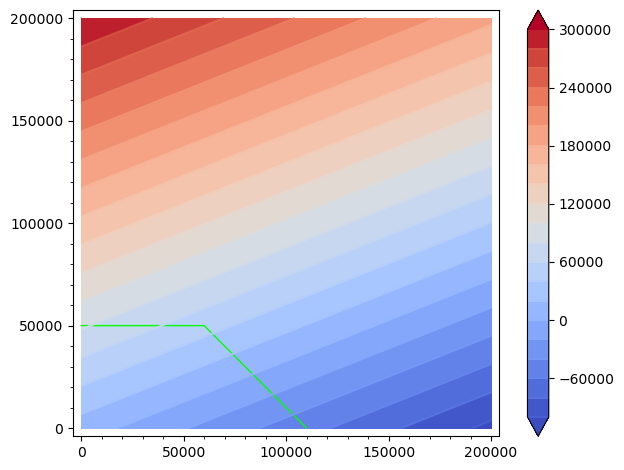
\includegraphics[width=\linewidth]{ex_1_profits.png}
    \caption{Contour plot of the profit function with the linear constraint function in green.}
\end{figure}



\newpage

    \label{ex:2}
    \begin{minted}{python}
# Show that the pig is gaining weight at 5 lbs / day at t = 0:
w(t) = 800 / (1 + 3 * (math.e)^(-t/30))
w_prime(t) = w.derivative(t)
w_pprime(t) = w_prime.derivative(t)
w_ppprime(t) = w_pprime.derivative(t)

print(f"At t=0, the pig is gaining {w_prime(0)} lbs per day")

# Calculate as t gets large
# t_0 = 3 # bad guess; close to crit point
t_0 = 30
guesses=[t_0]

for i in range(10):
    t_0 = t_0 - w_pprime(t_0) / w_ppprime(t_0)
    guesses.append(t_0)
    
root = round(guesses[-1], 2)
print(f'There is a root at {root}. It corresponds to maximum growth rate of {round(w_prime(root),3)}.')


# Returns:
# At t=0, the pig is gaining 5.0 lbs per day
# There is a root at 32.96. It corresponds to maximum growth rate of 6.667.
    \end{minted}

    \captionof{listing}{Exercise 2 (a) Code}
    
\newpage



    \label{ex:3}
    \begin{minted}{python}
# new pig problem
t = var('t')  # time in days

# Parameters
w0 = 200   # init weight of pig
rw = 5     # growth rate of pig (lb/day)
m0 = 0.65  # init market price ($/pound)
rm = -0.01 # market price rate of change ($/lbs/day)
d  = 0.45  # daily cost to keep the pig

# Functions
w(t) = 800 / (1 + 3 *(math.e)^(-t/30))   # weight of pig
m(t) = m0 + rm*t   # market price
r(t) = w(t)*m(t)   # revenue
c(t) = d*t         # cost
p(t) = r(t) - c(t) # profit

# Solve the Model
pprime    = p.derivative(t)        # derivative of profit
ppprime = pprime.derivative(t)

t_0 = 2
guesses=[t_0]
for i in range(10):
    t_0 = t_0 - pprime(t_0) / ppprime(t_0)
    guesses.append(t_0)

root = guesses[-1]
print(guesses)
print(f"There is a root at {root}. It corresponds to a profit of ${p(root)}.")
show(plot(pprime(t), 0, 20))
show(plot(p(t),0,20))

# Returns:
# There is a root at 12.33. It corresponds to a profit of $135.42.
    \end{minted}

    \captionof{listing}{Exercise 2 (b) Code}
    

\newpage

\label{ex:4}
\begin{minted}{python}
# Variables
x = var('x') # sub price
y = var('y') # ad price

# Parameters
subs_0 = 80_000  # current subscribers (subscriber / week)
ads_0  = 350     # current ads (pages / week)
d_p_ad  = 250    # dollars per advertisement
d_p_pap = 1.50   # dollars per paper (per subscriber)

slope_price_subs = -50000 # -5000 subs per $0.10
slope_price_ads = -0.5    # -50 pages per $100
slope_ads_subs = 20       # 20 subs per page

# Equations
A(y) = ads_0 + slope_price_ads * (y - d_p_ad)
S(x, y) = subs_0 + slope_price_subs * (x - d_p_pap) + slope_ads_subs * (A(y) - ads_0)
z(x, y) = (x * S(x, y)) + (y * A(y))

#first derivatives
F(x,y) = z.derivative(x)
G(x,y) = z.derivative(y)

print(f"{F=}")
print(f"{G=}")

#Second derivatives
F_x(x,y) = F.derivative(x)
F_y(x,y) = F.derivative(y)
G_x(x,y) = G.derivative(x)
G_y(x,y) = G.derivative(y)

print(f"{F_x=}")
print(f"{F_y=}")
print(f"{G_x=}")
print(f"{G_y=}")
\end{minted}

    \captionof{listing}{Exercise 3 (b) Code}

    \newpage

\label{ex:5}
\begin{minted}{python}
OF(x,y) = [F(x,y), G(x,y)]


def df(v):
    (x,y) = v
    return Matrix([grad(j)(x,y) for j in OF])

X = vector([1.5, 350])

guesses=[X]
for i in range(5):
    (x,y) = X
    X = X - df(X).inverse() * OF(x,y)
    guesses.append(X)
    
print(guesses)
print(f'There is a solution at approximately {guesses[-1]}')
\end{minted}
\captionof{listing}{Exercise 3 (c)}

\end{document}